\documentclass{article}
\usepackage[utf8]{inputenc}
\usepackage[version=4]{mhchem}
\usepackage{tikz, tcolorbox}
\usepackage{setspace}
\usepackage{siunitx}
\title{CHEM IA DRAFT}
\author{Peter Wang}
\date{November 2021}

\usepackage{geometry}
 \geometry{
 a4paper,
 total={170mm,257mm},
 left=20mm,
 right=20mm,
}

\begin{document}
\maketitle
\section{Introduction}
Ever since I immigrated to Canada as a child, it has become my family’s tradition to visit a new ski resort every winter. However, I observed over the years that when I brought my phone along to take pictures of the landscape, it would immediately shutdown as soon as I took it out of my coat pocket. When I tried to restart the device, it would indicate that the device had no battery even though I had fully charged it beforehand. I later learned in high school that a battery is simply a device that stores electrical energy in the form of chemical energy and converts the stored energy into electrical energy when the battery is being used through a chemical reaction. During our thermodynamics unit, we learned about the concept about spontaneous and non-spontaneous reactions. In a non-spontaneous reaction, additional energy is required to continue the reaction, whereas a spontaneous reaction does not require external energy. The spontaneity of a reaction is indicated by a variable known as the Gibbs Free Energy of reaction. This led me to wonder how the temperature at which a reaction took place affected the Gibbs Free Energy of the reaction.

\section{Investigation}
\subsection{Reaction Under Study}
The reaction studied in this investigation is the dissolution of Ammonium Nitrate within water, which produces Ammonium cations and Nitrate anions. The reaction was chosen for this investigation as Ammonium Nitrate is rather affordable and the reaction is very endothermic, hence a small quantity can produce a noticeable temperature change. 
\begin{equation}
\ce{NH4NO3 (s) ->[H2O (l)] NH4+ (aq) + NO3- (aq)}
\end{equation}
Furthermore, this reaction was chosen because the enthalpy

\subsection{Research Question}
\textit{The effect of absolute temperature on the Gibbs Free Energy of the dissolution of Ammonium Nitrate in Water at 298K, 303K, 308K, 313K and 318K.}

\subsection{Background Information}
The Gibbs Free Energy of a reaction ($\Delta G$) is a single state function that combines the enthalpy and entropy of reaction and is used to indicate the amount of available energy that can be used to do work. The Gibbs Free Energy value is measured in Joules and can be calculated by taking the difference between the enthalpy ($\Delta H$) of the reaction and the product of the entropy ($\Delta S$) and absolute temperature ($T$). The Gibbs Free Energy of a reaction is used to predict the spontaneity of the reaction.  If the $\Delta G > 0$, then the reaction is non-spontaneous, and the reverse is true where if $\Delta G < 0$, then the reaction is spontaneous. When the $\Delta G = 0$, the system is in equilibrium and there will be equal concentrations of reactants and products. As indicated by the equation \ref{eq:5}, the Gibbs Free Energy of a chemical reaction varies based on the temperature in which it occurs, hence a reaction could be spontaneous at a temperature value but non-spontaneous at another. 
\begin{equation}
\mathrm{\Delta G = \Delta H - T \Delta S } \label{eq:5}
\end{equation}
Furthermore, both the enthalpy and entropy of a chemical reaction are also temperature dependent values. The enthalpy of a reaction is temperature dependent as it is given as the difference of enthalpy of formation between the specific enthalpy of the product and reactants. 
\begin{equation}
\ce{\Delta H = \sum{\Delta H_{products}} - \sum{\Delta H_{reactants}}} \label{eq:9}
\end{equation}
As temperature is increased, molecules have more excited vibrational and rotational quantum numbers. This in turn increases the rotational and vibrational quantum numbers, and hence less energy is required to break the existing bonds. Moreover, according to Kirchhoff's Law of thermodynamics, the temperature dependence of the enthalpy of reaction's dependence on temperature is given by formula \ref{eq:8} below. As the specific heat capacity is usually not constant, it is given as a function over temperature. Therefore, the enthalpy of reaction at a specific absolute temperature value can be given as the sum between the initial enthalpy value ($\ce{H_{T_i}}$) and the integral of the specific heat capacity function ($\ce{c_p}$) between $\ce{T_i}$ and $\ce{T_f}$
\begin{equation}
\ce{H_{T_f} = H_{T_i}} + \int_{\mathrm{T_{i}}}^{\mathrm{T_{f}}} \mathrm{c_p dT} \label{eq:8}
\end{equation}
If the specific heat capacity is temperature independent over a specific temperature range, the equation above can be further simplified. Literature values suggests that the specific heat capacity of water remains measurably constant in liquid state ($\ce{273.15K, 373.15K}$), sufficiently covering the temperature range investigated in this paper.
\begin{equation}
\ce{H_{T_f} = H_{T_i} + \mathrm{c_p(T_f - T_i)}} \label{eq:1}
\end{equation}
Likewise, the entropy of a reaction is also dependent on the temperature at which the reaction occurs. The Entropy of Reaction is given as the difference between the sum of the Entropies of the products and the sum of the Entropies of the reactants. 
\begin{equation}
    \ce{\Delta S = \sum{\Delta S_{products}} - \sum{\Delta S_{reactants}}} \label{eq:10}
\end{equation}
\noindent
Molecules at higher absolute temperature values possess greater kinetic energy compared to molecules at lower absolute temperature values. Consequently, they have greater disorder and hence a higher absolute entropy value. The temperature dependence of entropy change at constant pressure is given by the following equation. If the specific molar heat capacity of the reaction is known, then the entropy of reaction at constant pressure for any given temperature is the product between the number of moles of reactants ($\ce{n}$), the molar specific heat capacity ($\ce{c_p}$) and the nature logarithm of the final temperature over the initial temperature.
\begin{equation}
\ce{\Delta S = nC_p \ln{\frac{\mathrm{T_2}}{\mathrm{T_1}}}|_p} \label{eq:2}
\end{equation}
The Gibbs Free Energy at a temperature value can be theoretically calculated by utilizing equations \ref{eq:1} and \ref{eq:2}. However, a much simpler method for calculating the theoretical Gibbs Free Energy value at constant pressure would be to implement the Gibbs-Helmholtz Equation. The Gibbs-Helmholtz equation provides the direct relationship between the enthalpy of reaction and the Gibbs Free Energy of reaction, as it does not involve the entropy of reaction variable. The equation can be derived from equation \ref{eq:5} as shown in the derivation below.
\begin{equation}
\begin{split}
\ce{
\Delta G &= \Delta H - T \Delta S \\ 
\frac{\Delta G}{T} &= \frac{\Delta H}{T} - \Delta S \\ 
\frac{\partial (\Delta G/T)}{\partial T}|_p &= \frac{1}{T} \frac{\partial H}{\partial T}|_p - \frac{H}{T^2} - \frac{\partial S}{\partial T}|_p \\ 
&= \frac{c_p}{T} - \frac{H}{T^2} - \frac{c_p}{T} \\ 
&= -\frac{H}{T^2}
}
\end{split}
\end{equation}
The Gibbs-Helmholtz equation in its raw form is given by equation \ref{eq:3} below, where the partial derivative of the Gibbs Free Energy on temperature is given as the negative quotient of the enthalpy of reaction divided by the square of the absolute temperature.
\begin{equation}
\ce{(\frac{\partial(\Delta G/T)}{\partial T})|_p = - \frac{\Delta H}{T^2}} \label{eq:3}
\end{equation}
If the $\Delta G$ value at a given temperature ($\ce{T_i}$), such as under SATP (standard ambient temperature and pressure) conditions given in the IBO data-booklet is known, the $\Delta G$ value at any other temperature ($\ce{T_f}$) can be calculated by integrating the equation \ref{eq:3}. The integration process is shown below in equation \ref{eq:4}. However, the $\Delta H$ value is not constant, but as a function over temperature as the enthalply is also temperature dependent as mentioned previously.
\begin{equation}
\begin{split}
\int_{\Delta \mathrm{G(T_i)/T_i}}^{\mathrm{\Delta G(T_f)/T_f}}{(\frac{\mathrm{\partial (\Delta G/T)}}{\mathrm{\partial T}})|\ce{_p dT}} &= \frac{\mathrm{\Delta G(T_f)}}{\mathrm{T_f}} + \frac{\mathrm{\Delta G(T_i)}}{\mathrm{T_i}} \label{eq:4} \\
&= -\int_{\mathrm{T_i}}^{\mathrm{T_f}} \frac{\mathrm{\Delta H}}{\mathrm{T^2}} dT 
\end{split}
\end{equation}

\subsection{Calculation of SATP Values}
To determine the change of the Gibbs Free Energy based on temperature, the Enthalpy and Entropy of reaction under SATP conditions must first be calculated. Conveniently, as the reaction involves dissolving Ammonium Nitrate in water, the enthalpy is given as an Enthalpy of Solution value, which can be found to be $\ce{25.69 kJ/mol}$ in Table 19 of the IB Data-Booklet. The Entropy of reaction can be calculated using equation \ref{eq:10}.
\begin{tcolorbox}[title=Calculation of Entropy of Reaction under SATP Conditions ($\Delta S^{\theta}$)]
\begin{equation}
    \begin{split}
        \mathrm{\Delta S} &= \sum{\mathrm{\Delta S_{products}}} - \sum{\mathrm{\Delta S_{reactants}}} \\
        &= \mathrm{(113.4 J/mol K + 146.4 J/mol K) - (151.1 J/mol K)} \\
        &= \mathrm{108.7 J/mol K}
    \end{split}
\end{equation}
\end{tcolorbox}
\noindent
The positive Entropy of reaction value calculated can be verified as the reaction involves solid Ammonium Nitrate dissolving to form dissociated ions, which have are more disordered than the solid. Therefore, since the products are more disordered than the reactant, the entropy of reaction will also be positive. \\ \\

From the Enthalpy and Entropy of reaction, the Gibbs Free Energy of reaction can be calculated equation \ref{eq:5}.
\begin{tcolorbox}[title=Calculation of the Gibbs Free Energy under SATP Conditions ($\Delta G^{\theta}$)]
\begin{equation}
    \begin{split}
        \mathrm{\Delta G^{\theta}} &= \mathrm{\Delta H^{\theta}} - \mathrm{T \Delta S^{\theta}} \\
        &= 25.69 \mathrm{kJ/mol} - 298.15\mathrm{K} \times 108.7 \mathrm{J/mol K} \\
        &= -6.72 \mathrm{kJ/mol}
    \end{split}
\end{equation}
\end{tcolorbox}

\subsection{Experimental Methodology}
This paper investigates the effect of absolute temperature on the Gibbs Free Energy of the reaction by measuring the enthalpy of reaction at various absolute temperature values. The enthalpy of reaction will be measured through the use of a coffee cup calorimeter, which measures the heat flow in a chemical reaction. The calorimeter is simply an insulated container, with the lid to act as the system for the chemical reaction to occur. When the chemical reaction occurs, the heat of the reaction is absorbed by or extracted from the water and the temperature of the water will change. The change in temperature is measured by a thermometer, which will be used to calculate the enthalpy change of the reaction using the heat flow equation as given by equation \ref{eq:6} below.
\begin{equation}
\ce{q = mc_{\mathrm{p}} \Delta T} \label{eq:6} 
\end{equation}
As the enthalpy of the reaction is negative to the heat absorbed/gained by the water, the reaction enthalpy can be given as the negative of the heat transfer to the water as shown in equation \ref{eq:7}
\begin{equation}
\ce{\Delta H = -q} \label{eq:7}
\end{equation}
Due to the fact that a coffee cup does not have perfect built in insulation, therefore, for an endothermic reaction, the system will gain heat from the surroundings and alter the final temperature value. To account for the heat loss to the environment, after the reaction has concluded, the Pasco-Thermometer will continue to measure the rate of temperature gain from environment. The rate can then be used to graphically extrapolate the corrected final temperature of the reaction, which would be the temperature value reached assuming that the coffee cup calorimeter was a closed system. 

\section{Variables}
\subsection{Independent Variable}
The independent variable of this investigation is the \textbf{absolute temperature }($\ce{K}$). In equation \ref{eq:5}, the three variables that are used to calculate the Gibbs Free Energy of a reaction are the enthalpy of reaction, entropy of reaction and absolute temperature. As stated previously, both the enthalpy and entropy of reaction regardless of temperature, only changes if the reactants were changed. Hence, the absolute temperature was chosen to be the independent variable of the investigation. The temperature values tested were 298K, 303K, 308K, 313K and 318K as the use of five different temperatures values increases the reliability of the experimental results. 

\subsection{Dependent Variable}
The dependent variable of the investigation is the \textbf{enthalpy of the reaction}($\ce{kJ/mol}$) which will be measured through the use of a coffee cup calorimeter. Referencing equation \ref{eq:4}, the Gibbs Free Energy can be calculated if the enthalpy and entropy of reaction are known as the temperature is the independent variable of the investigation. Only the enthalpy reaction can be directly measured experimentally, and hence was chosen for the purpose of this investigation. The entropy of reaction will be calculated using the equation \ref{eq:2} using the theoretical values provided in the IBO data-booklet. It is important to note that the enthalpy values will be measured in units of ($\ce{kJ/g}$, however, the units will be converted to ($\ce{kJ/mol}$) as all of the other calculations will be calculated in terms of moles.

\subsection{Controlled Variables}
\subsubsection{Coffee Cup Calorimeter}
The same coffee cup calorimeter must be used for all of the trials as different calorimeters have different insulation, hence different heat loss to environment. This will affect the measured enthalpy of reaction as a calorimeter with greater insulation will measure a larger temperature change, whereas a calorimeter will little to no insulation will measure a small change in temperature.

\subsubsection{Amount of Reactants}
The amount of reactants must be kept constant between trials. If the volume of water were to be altered, then the same amount of energy will produce a different temperature change. As indicated by equation \ref{eq:6}, the heat transfer is equal to the product between the mass, specific heat capacity and temperature. Therefore, if the mass of water were to increase, then the change in temperature will decrease, and the reverse is true as well where if the mass of the water were to decrease, the temperature change would increase. Furthermore, the number of moles of Ammonium Nitrate must also be kept constant as the enthalpy of reaction is based off the number of moles reacted.

\subsubsection{Temperature of Surroundings}
The temperature of the surroundings must be kept constant throughout all of the trials as different surrounding temperatures will result in different heat gain/lost to environment. Therefore, the experiment must be conducted in the same area of the lab as even different areas within a room can have different temperature values. The room temperature should be kept constant and this is verified using a classroom thermometer.

\subsubsection{Even Distribution of Temperature within Water}
The temperature of the water must be even distributed to ensure that the effect of temperature on enthalpy of reaction is accurate. If only certain parts of the water was heated up to the desired temperatures, then the measured data values would be inconclusive.

\section{Experimental Method}
\subsection{Apparatus}
\begin{itemize}
    \item 165.0 g Ammonium Nitrate 
    \item 750 mL Distilled Water
    \item Insulated Coffee Cup (with Lid)
    \item Pasco-Thermometer
    \item Laptop with Bluetooth Connection
    \item Scrap Paper
    \item Stirring Rod
    \item Electronic Balance 
    \item Hot Plate
\end{itemize}

\subsection{Experimental Procedure}
\begin{enumerate}
    \item Measure 11.0 g of Ammonium Nitrate in a Paper weighing boat on a two digit electronic balance. 
    \item Measure 50 mL of water using a 50 mL Graduated Cylinder.
    \item Heat up the water to 25°C using a Electronic Hot Plate and verify that the temperature was reached using a Pasco-Thermometer.
    \item Pour the heated water into the coffee cup calorimeter and add the measured Ammonium Nitrate into the coffee cup.
    \item Immediately close the lid to the coffee cup and insert the Pasco-Thermometer and start recording the temperature changes in the SparkVue software.
    \item Once the temperature stops decreasing, let the Pasco-Thermometer to continue recording the temperature change for another 10 seconds.
    \item Repeat steps 1-7 for three trials at 30°C, 35°C, 40°C, 45°C and 50°C.
\end{enumerate}

\subsection{Risk Assessment}
\subsubsection{Safety Consideration}
Ammonium Nitrate is a strong oxidizer and is extremely explosive when exposed to high temperatures. Therefore, to ensure the safety of the experiment, the Ammonium Nitrate was placed in water of maximum temperature of 50°C, over 100°C less than the temperature at which Ammonium Nitrate begins to decompose. 
\subsubsection{Ethical Consideration}
There were no ethical considerations taken into account.
\subsubsection{Environmental Consideration}
Concentrated Ammonium Nitrate and Water solution should not be disposed within the drain. Therefore, the product solution must be diluted before being poured down the drainage system.

\subsection{Experimental Setup}
The experimental setup can be demonstrated by the picture below:

\section{Data Collection}
\subsection{Raw Data}


\subsection{Qualitative Observations}

\section{Data Processing}
\subsection{Sample Calculation}
The data processing procedure is demonstrated below through the use of a sample calculation. The data used in the sample trial is the data collected during trial one of the independent variable at the temperature of $\ce{303K}$. The raw data is shown in the table below.

\textbf{\underline{Table 1: Temperature of Water with Relationship to Time for Trial one at $T = 303K$}}
\begin{doublespace}
\begin{center}
\begin{tabular}{ |c|c| } 
 \hline
 $\ce{Time}($\mathrm{s}$)(\pm 0.1\mathrm{s})$ & $\ce{Temperature}(\mathrm{K})(\pm 0.01 \mathrm{K})$  \\ 
 \hline
 0 & 303.53  \\ 
 2 & 302.59  \\ 
 4 & 301.72 \\
 6 & 301.01 \\
 8 & 300.58 \\
 10 & 300.33 \\
 12 & 300.30 \\
 14 & 300.35 \\
 16 & 301.02 \\
 18 & 301.69 \\
 20 & 302.41 \\ 
 22 & 303.18 \\
 \hline
\end{tabular}
\end{center}
\end{doublespace}

\noindent
The measured variable of this investigation is the temperature change of the reaction, which is then implemented to calculate the enthalpy of reaction. However, as mentioned previously, the final temperature is influenced by the imperfect insulation of the coffee cup. Due to the endothermic nature of the reaction, to account for the heat gained from the surroundings, the rate of heat gain can be determined graphically, as shown by the graph below.

\begin{center}
\textbf{\underline{Figure 1: Extrapolation of Rate of Temperature Gain from Surroundings}}
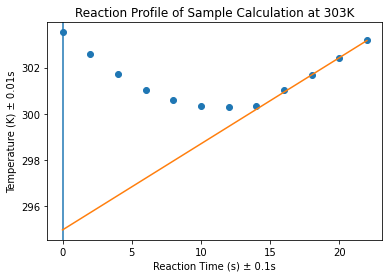
\includegraphics{SampleCalculation.png}    
\end{center}


\noindent
As can be seen in the graph, the temperature gain from the environment is determined graphically by drawing a line of best fit through the temperature values. By retracing the line back to the start of the reaction, when reaction time was at $\ce{0s}$, the corrected final temperature can be determined from the graph above to be $\ce{294.98K}$. The corrected final temperature has been determined, the temperature change ($\ce{\Delta T}$) can be determined as the difference between the final and initial temperature values.
\begin{tcolorbox}[title=Calculation of Temperature Change ($\ce{\Delta T}$)]
\begin{equation}
    \begin{split}
        \ce{
        \Delta T = &= T_{final} - T_{initial} \\
        &= 294.98 \pm 0.01 \si{K} - 303.53 \pm 0.01 \si{K} \\
        &= -8.55 \pm 0.02 K
        }
    \end{split}
\end{equation}

\end{tcolorbox}

\noindent
From the temperature value, the enthalpy of reaction can be calculated by using equation \ref{eq:6} to determine the heat transfer to the water and then implementing \ref{eq:7} to get the enthalpy of reaction.
\begin{tcolorbox}[title=Calculation of Enthalpy of Reaction ($\ce{\Delta H}$)]
\begin{equation}
    \begin{split}
        \ce{
        q &= mc_p \Delta T \\ 
        &= 100.0 \si{g} \times} \ce{4.18 \si{J/g.K}\times (-8.55 K \pm 2.3 \%) \\
        &= -3.6 kJ \pm 2.3\% \\
        \Delta H &= -q \\ 
        &= -(-3.6 kJ \pm 2.3\%) \\ 
        &= 3.6 kJ \pm 2.3\%
        }
    \end{split}
\end{equation}
\end{tcolorbox}
\noindent
The enthalpy of reaction calculated is determined to be a positive value, which validates the endothermic nature of the reaction. Furthermore, the experimental value can be compared to the literature value to ensure that it is approximately the same. \\ \\

\noindent
The enthalpy of solution of Ammonium Nitrate can be found in Table 19 of the IB Data-booklet, given to be $\ce{25.69 kJ/mol}$. The molar mass of $\ce{NH4NO3}$ can be calculated from the molar mass of the molecules based on values in Table 6 of the IB Data-Booklet.
\begin{tcolorbox}[title=Calculation of Molar Mass of $\ce{NH4No3}$]
\begin{equation}
    \begin{split}
        \ce{
        NH4NO3 &= 2 mol \times N + 4 mol \times H + 3mol \times O \\
        &= 2 mol \times} \ce{14.01 \si{g/mol} + 4mol \times} \ce{1.01 \si{g/mol} + 3mol \times} \ce{16.00 \si{g/mol} \\
        &= 80.06 \si{g/mol}
        }
    \end{split}
\end{equation}
\end{tcolorbox}
\noindent
In this investigation, $\ce{10.0 \pm 0.1 g}$ of Ammonium Nitrate is reacted in each trial, therefore the theoretical enthalpy of reaction should be given as percentage molar mass multiplied by the enthalpy of solution.
\begin{tcolorbox}[title=Calculation of Theoretical Enthalpy of Reaction ($\ce{\Delta H_{Theoretical}}$)]
\begin{equation}
\begin{split}
  \ce{
  \Delta H_{Theoretical} &= \frac{Mass of Reactant}{Molar Mass of NH4NO3} \times Enthalpy of Reaction \\
  &= \frac{11.0 g \pm 1.0\%}{80.06 g/mol} \times} \ce{25.69 kJ/mol \\
  &= 3.53 kJ/mol \pm} \ce{1.0\% g
  }  
\end{split}
\end{equation}
\end{tcolorbox}
\noindent
The theoretical enthalpy of reaction is $\ce{3.21 kJ \pm 1.0\%}$, which is fairly close to the theoretical value, which demonstrates that the experimental procedure is rather accurate. To calculate the molar enthalpy of reaction, the enthalpy of reacting $\ce{10.0g}$ can divide the molar mass of Ammonium Nitrate as shown below.
\begin{tcolorbox}[title=Calculation of Molar Enthalpy of Reaction ($\ce{\Delta H_{Molar}}$)]
\begin{equation}
    \begin{split}
        \ce{
        \Delta H_{Molar} &= 3.6 kJ \div \frac{11.0 g \pm 1\%}{80.06 g/mol} \\ 
        &= 26.2 kJ/mol \pm 2.3\%
        }
    \end{split}
\end{equation}
\end{tcolorbox}
\noindent
To calculate the theoretical entropy value, equation \ref{eq:2} where the change in entropy based on temperature is given as the molar specific heat capacity multiplied by the natural logarithm of the final temperature divided by the initial. The initial temperature in this case would be the temperature in which the IB data-booklet values were recorded, which would be under SATP conditions at $\ce{298.15K}$.
\begin{tcolorbox}[title=Calculation of Entropy Change from Temperature ($\ce{\Delta S_{Change}}$)]
\begin{equation}
    \begin{split}
        \ce{ 
        \Delta S_{Change} &= nC_p \ln \frac{T_{final}}{T_{Initial}} \\
        &= \frac{11.0 g \pm 1.0\%}{80.06 g/mol} \times} \ce{139.30 J/mol K \times \ln \frac{303K}{298.15K} \\
        &= 0.31 J/mol k \pm 1.0\%
        }
    \end{split}
\end{equation}
\end{tcolorbox}

\noindent
Therefore, to calculate the entropy of reaction at $\ce{303K}$, the change in entropy based on temperature can simply be added to the entropy at $\ce{298.15K}$. This is shown in the calculations below.

\begin{tcolorbox}[title=Calculation of Entropy of Reaction at $\ce{303K}$ ($\ce{\Delta S_{T_{final}}})$]
\begin{equation}
    \begin{split}
        \ce{
        \Delta S_{T_{final}} &= \Delta S_{T_{Initial}} + \Delta S_{Change} \\
        &= 108.7 J/mol K + 0.31 J/mol K \pm 1.0\% \\
        &= 109.1 J/mol K \pm 1.0\%
        }
    \end{split}
\end{equation}
\end{tcolorbox}

\noindent
After both the enthalpy and entropy has been determined, the Gibbs Free Energy of the reaction at $\ce{303K}$ can be determined by utilizing equation \ref{eq:5}.

\begin{tcolorbox}[title=Calculation of Gibbs Free Energy at $\ce{303K}$ ($\ce{\Delta G_{T_{final}}}$)]
\begin{equation}
    \begin{split}
        \ce{
        \Delta G_{T_{final}} &= \Delta H_{T_{final}} - T_{final} \Delta S_{T_{final}} \\
        &= 26.2 kJ/mol \pm 2.3\% - 303K \times} \ce{109.01 J/mol K \pm 1.0\% \\ 
        &= -6.83 \mathrm{kJ} \pm 2.3\%
        }
    \end{split}
\end{equation}
\end{tcolorbox}

\noindent
This process can be repeated for every other trial and the Gibbs Free Energy at every absolute temperature can be determined. This sample calculation also demonstrated the error calculation involved with the uncertainty of the equipment involved in this investigation. \\ \\

\noindent
The experimental values can be compared with the literature values through the use of the Gibbs-Helmholtz equation. The change in Gibbs Free Energy from the literature value at $\ce{298.15K}$ to the experimental value at $\ce{303K}$ can be theoretically calculated using equation \ref{eq:4}.
\begin{tcolorbox}[title=Calculation of Theoretical Gibbs Free Energy Change from Temperature ($\ce{\Delta G_{Change}}$)]
\begin{equation}
    \begin{split}
        \int_{\Delta \mathrm{G(T_i)/T_i}}^{\Delta \mathrm{G(T_f)/T_f}}{(\frac{\mathrm{\partial (\Delta G/T)}}{\mathrm{\partial T}})\ce{|_p dT}} &= -\int_{\mathrm{T_i}}^{\mathrm{T_f}} \frac{\mathrm{\Delta H}}{\mathrm{T^2}} dT \\
        &= -\int_{298.15 \mathrm{K}}^{303\mathrm{K}} \frac{\ce{\Delta H_{Experimental} - \Delta H_{Literature}}}{\ce{(T_{final} - T_{initial}})^2} dT \\
        &= -\int_{298.15\mathrm{K}}^{303\mathrm{K}} \frac{28.8 \mathrm{kJ/mol} - 25.7 \mathrm{kJ/mol}}{(303\mathrm{K} - 298.15\mathrm{K})^2} \\
        &= -0.64 \mathrm{KJ/mol}
    \end{split}
\end{equation}
\end{tcolorbox}
\noindent
From the theoretical Gibbs Free Energy change value, the Gibbs Free Energy of the reaction at $\mathrm{303K}$ can be determined to be the sum of the literature value at $\mathrm{298.15K}$ an the Gibbs Free Energy change value.
\begin{tcolorbox}[title=Calculation of Theoretical Gibbs Free Energy at $\mathrm{303K}$]
\begin{equation}
    \begin{split}
        \mathrm{\Delta G_{303K}} &= \mathrm{\Delta G_{Literature}} + \mathrm{\Delta G_{Change}} \\ 
        &= -6.72 \mathrm{kJ/mol} + (-0.64 \mathrm{kJ/mol}) \\
        &= -7.36 \mathrm{kJ/mol}
    \end{split}
\end{equation}
\end{tcolorbox}
The percentage error of this investigation is given by the following formula.
\begin{tcolorbox}[title=Calculation of Percentage Error ($\mathrm{\% Error}$)]
\begin{equation}
    \begin{split}
    \% Error &= \frac{\mathrm{|\Experimental - Theoretical|}}{\mathrm{\Theoretical}} \times 100 \% \\
    &= \frac{|-6.83 \mathrm{kJ/mol} - (-7.36 \mathrm{kJ/mol}|}{|-7.36 \mathrm{kJ/mol}|} \times 100 \% \\
    &= 7.2 \%
    \end{split}
\end{equation}
\end{tcolorbox}

\subsection{Processed Data}

\subsection{Evaluation of Data}

\section{Evaluation}
\subsection{Strengths}
The investigation proved to be rather successful 

\subsection{Weaknesses} 
\subsubsection{Assumption of Constant Specific Heat Capacity} \label{subsection1}
This investigation assumed that the specific heat capacity of the water remained constant regardless of the temperature which is untrue as the specific heat capacity of water increases when temperature is increased. Therefore, this decreased the calculated value of the enthalpy of reaction at higher temperatures.

\subsubsection{Imperfectly Insulated Container}
Due to the imperfect insulation of the Calorimeter, there was heat gained from the environment. Even though this issue was combated by extrapolating the heat gain from the surroundings graphically, the rate of heat gain is not perfectly accounted for and hence will cause discrepancies when calculating the enthalpy of reaction. To combat this issue, better insulated Calorimeters can be used to reduce the heat gain from the environment and lower the impact of the imperfectly insulated system. 

\subsection{Extensions}
\subsubsection{Temperature Dependence of Specific Heat Capacity}
As mentioned in section \ref{subsection1}, under the Weaknesses section of this investigation, the specific heat capacity of water is not constant. Therefore, a further extension to this investigation could include implementing the specific heat capacity as a function of temperature rather than as a constant value.

\subsubsection{Investigation of Phase Changes}
This investigation explored the effect of temperature on the Gibbs Free Energy where no phase changes were involved. However, if the reactants were heated to higher temperature, the effect of phase change on the Gibbs Free Energy of reaction can be explored.

\subsubsection{Gibbs Free Energy in Electro-Chemistry}
In this exploration, the effect of temperature on the Gibbs Free Energy of dissolving Ammonium Nitrate was explored. However, a possible extension would be to investigate the effect of absolute temperature on the Cell Potential using the Nernst equation.

\subsection{Scope Limitations}


\section{Conclusion}


\end{document}
